\documentclass[noinstructornotes]{ximera}
%handout:  for handout version with no solutions or instructor notes
%handout,instructornotes:  for instructor version with just problems and notes, no solutions
%noinstructornotes:  shows only problem and solutions

%% handout
%% space
%% newpage
%% numbers
%% nooutcomes

%I added the commands here so that I would't have to keep looking them up
%\newcommand{\RR}{\mathbb R}
%\renewcommand{\d}{\,d}
%\newcommand{\dd}[2][]{\frac{d #1}{d #2}}
%\renewcommand{\l}{\ell}
%\newcommand{\ddx}{\frac{d}{dx}}
%\everymath{\displaystyle}
%\newcommand{\dfn}{\textbf}
%\newcommand{\eval}[1]{\bigg[ #1 \bigg]}

%\begin{image}
%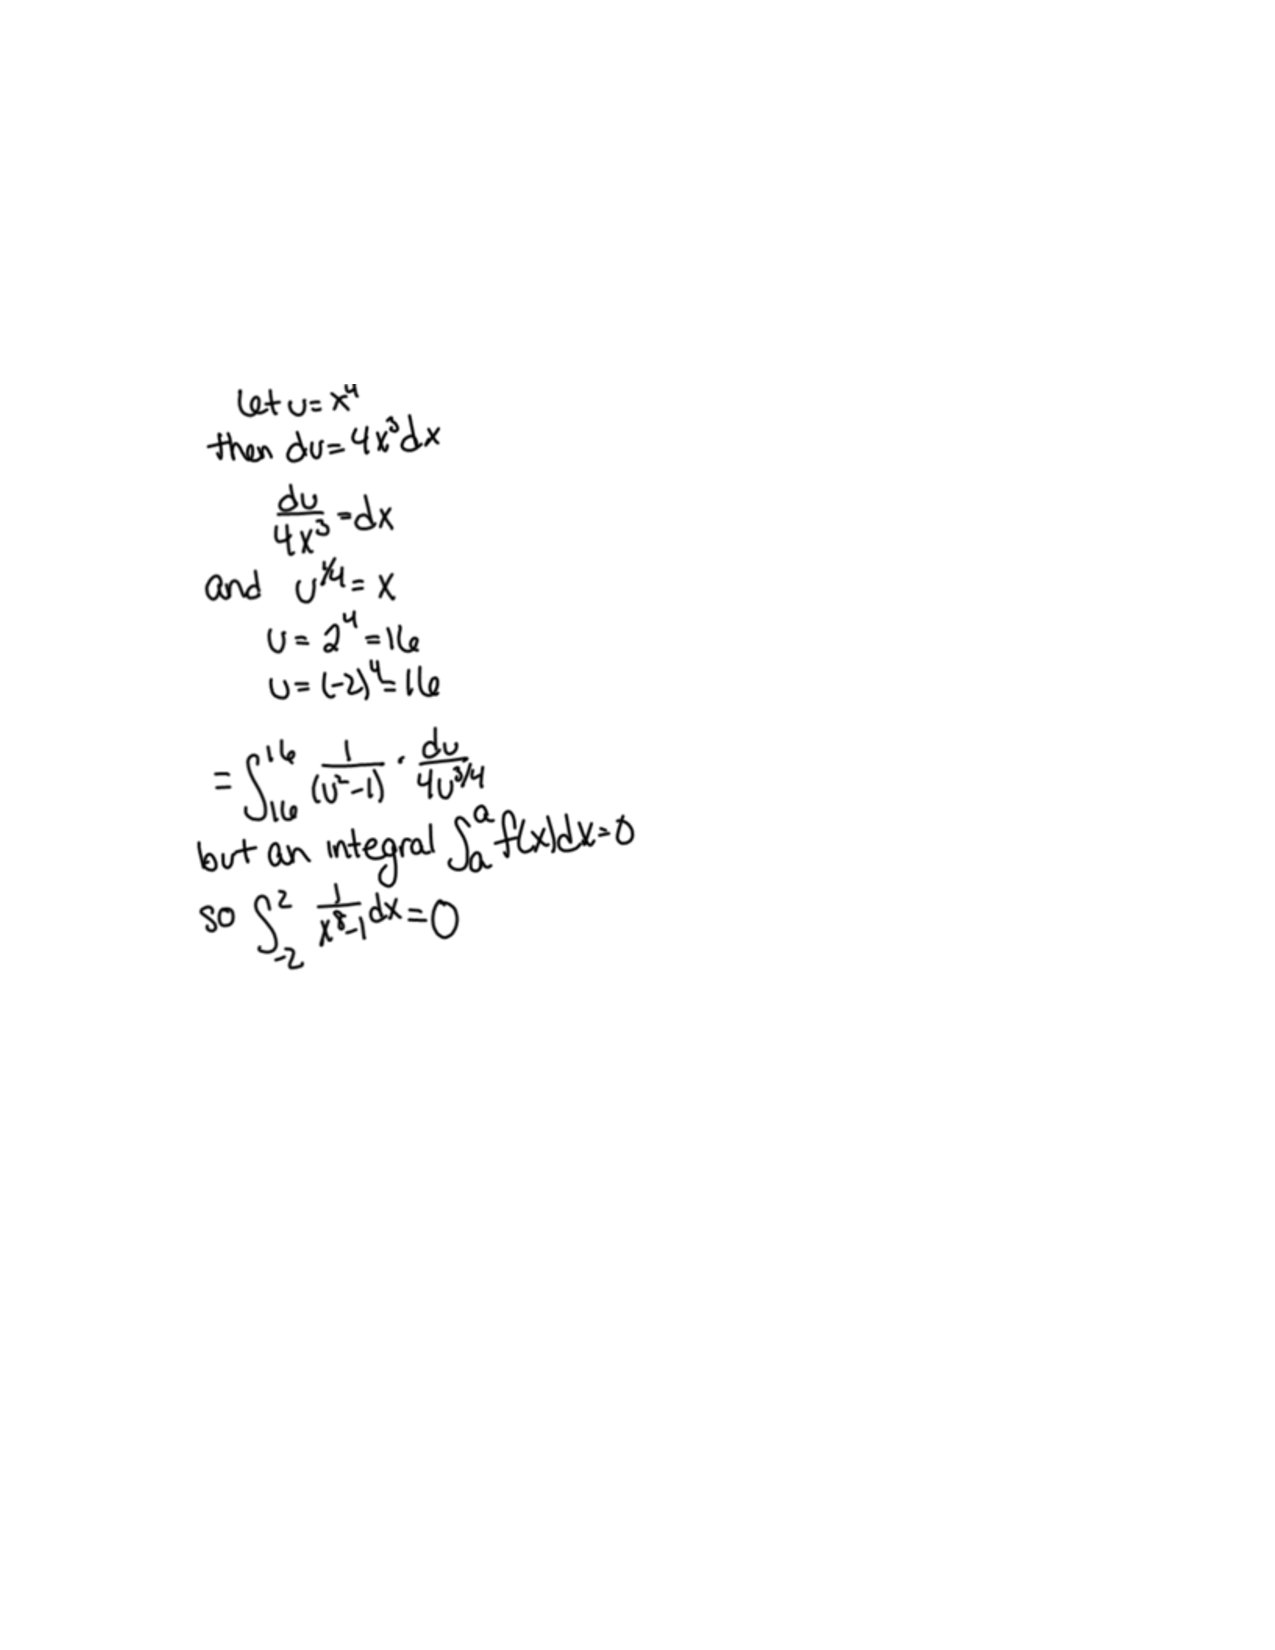
\includegraphics[trim= 170 420 250 180]{Figure1.pdf}
%\end{image}

%add a ``.'' below when used in a specific directory.
\newcommand{\RR}{\mathbb R}
\renewcommand{\d}{\,d}
\newcommand{\dd}[2][]{\frac{d #1}{d #2}}
\renewcommand{\l}{\ell}
\newcommand{\ddx}{\frac{d}{dx}}
\newcommand{\dfn}{\textbf}
\newcommand{\eval}[1]{\bigg[ #1 \bigg]}

\usepackage{multicol}

\renewenvironment{freeResponse}{
\ifhandout\setbox0\vbox\bgroup\else
\begin{trivlist}\item[\hskip \labelsep\bfseries Solution:\hspace{2ex}]
\fi}
{\ifhandout\egroup\else
\end{trivlist}
\fi} %% we can turn off input when making a master document

\title{Dot Products and Cross Products}
\begin{document}
\begin{abstract}		\end{abstract}
\maketitle



\section{Warm up:}



If $\vec{a}$, $\vec{b}$, and $\vec{c}$ are vectors in $3$-space $\mathbb{R}^3$, which of the following make sense?
	\begin{multicols}{3}
	\begin{enumerate}
	\item  $(\vec{a} \cdot \vec{b}) \cdot \vec{c}$
	\item  $(\vec{a} \cdot \vec{b})\vec{c}$
	\item  $(\vec{a} \times \vec{b}) \cdot \vec{c}$
	\item  $(\vec{a} \cdot \vec{b}) + \vec{c}$
	\item  $(\vec{a} \times \vec{b}) + \vec{c}$
	\item  $\vec{a} \cdot (\vec{b} + \vec{c})$
	\item  $\vec{a} \cdot (\vec{b} \times \vec{c})$
	\item  $\vec{a} \times (\vec{b} \cdot \vec{c})$
	\item  $(\vec{a} \times \vec{b}) \vec{c}$
	\end{enumerate}
	\end{multicols}
	
	\begin{freeResponse}
	\begin{enumerate}
	\item  Since $\vec{a} \cdot \vec{b}$ is a scalar, $(\vec{a} \cdot \vec{b}) \cdot \vec{c}$ does \dfn{not} make sense.
	\item  Now since $\vec{a} \cdot \vec{b}$ is a scalar, $(\vec{a} \cdot \vec{b})\vec{c}$ \dfn{does} make sense as regular scalar multiplication.
	\item  Since $\vec{a} \times \vec{b}$ is a vector, $(\vec{a} \times \vec{b}) \cdot \vec{c}$ \dfn{does} make sense.
	\item  This is of the form ``scalar + vector'', which does \dfn{not} make sense.
	\item  Since $\vec{a} \times \vec{b}$ is a vector, $(\vec{a} \times \vec{b}) + \vec{c}$ \dfn{does} make sense.
	\item  This is of the form ``vector $\cdot$ vector'', which \dfn{does} make sense.
	\item  This is also of the form ``vector $\cdot$ vector'', which \dfn{does} make sense.
	\item  This is of the form ``vector $\times$ scalar'', which does \dfn{not} make sense.
	\item  Since $\vec{a} \times \vec{b}$ is a vector, this does \dfn{not} make sense.
	\end{enumerate}
	\end{freeResponse}
	
\begin{instructorNotes}
This problem can be split up among the groups if the instructor likes (with maybe 3 or so per group).  
\end{instructorNotes}






\section{Group work:}

\begin{problem}
Answer the following questions about $\text{proj}_v u$.
	\begin{enumerate}
	\item  Is $\text{proj}_v u$ a vector of the form $c \vec{v}$ or $c \vec{u}$ (where $c$ is a real number)?  
	ie, is $\text{proj}_v u$ parallel to $\vec{u}$ or $\vec{v}$?  
	
	\item  If $\vec{u} = 5 \hat{\imath} + 6 \hat{\jmath} - 3 \hat{k}$ and $\vec{v} = 2 \hat{\imath} - 4 \hat{\jmath} + 4 \hat{k}$, find $\text{proj}_v u$.
	
	\item  For $\vec{u}$ and $\vec{v}$ from part (b), write $\vec{u}$ as the sum of two perpendicular vectors, one of which is parallel to $\vec{v}$.  Verify that the other vector is perpendicular to $\vec{v}$.
	\end{enumerate}
	
	\begin{freeResponse}
	\begin{enumerate}
	\item  $\boxed{c \vec{v}}$
	
	\item  
		\begin{align*}
		\text{proj}_v u 
		&= \frac{\vec{u} \cdot \vec{v}}{\vec{v} \cdot \vec{v}} \vec{v}  \\
		&= \frac{10-24-12}{4+16+16} \langle 2,-4,4 \rangle  \\
		&= \boxed{- \frac{13}{18} \langle 2,-4,4 \rangle  }
		\end{align*}
	
	
	
	\item  A schematic picture of the situation is as follows:
		\begin{image}
		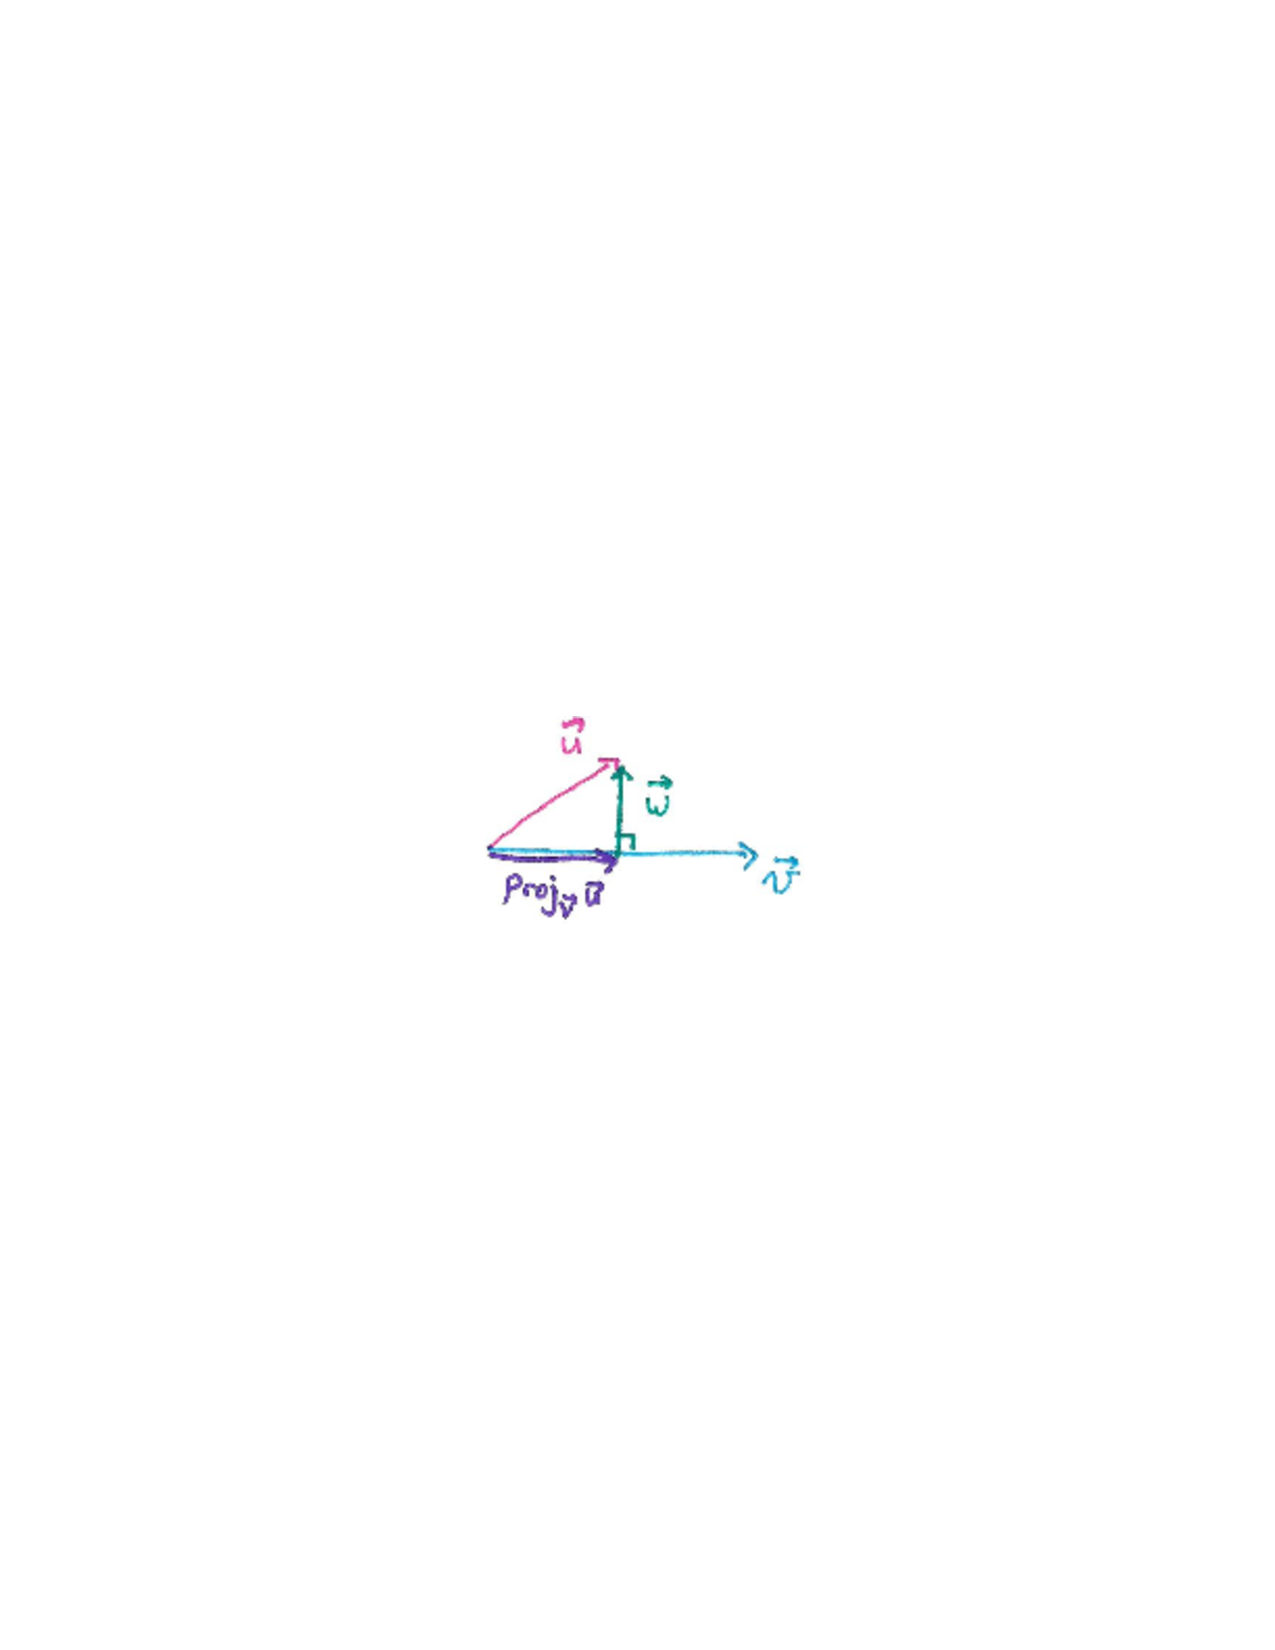
\includegraphics[trim= 170 350 170 350, scale=1]{Figure12-3-1.pdf}
		\end{image}
		
	The vector which is parallel to $\vec{v}$ is 
		\[
		\text{proj}_v u = \boxed{\left\langle - \frac{13}{9}, \frac{26}{9}, - \frac{26}{9} \right\rangle}
		\]
	The vector which is orthogonal to $\vec{v}$ is
		\begin{align*}
		\vec{w} := \vec{u} - \text{proj}_v u
		&= \left\langle 5,6,-3 \right\rangle - \left\langle - \frac{13}{9}, \frac{26}{9}, - \frac{26}{9} \right\rangle  \\
		&= \boxed{\left\langle \frac{58}{9}, \frac{28}{9}, - \frac{1}{9} \right\rangle}
		\end{align*}
	And, clearly, $\text{proj}_v u + \vec{w} = \text{proj}_v u + (\vec{u} - \text{proj}_v u) = \vec{u}$.  
	
	To verify that $\vec{w}$ is orthogonal to $\vec{v}$, we take the dot product and show we get 0. \\
	$\vec{w} \cdot \vec{v} = \left\langle \frac{58}{9}, \frac{28}{9}, - \frac{1}{9} \right\rangle \cdot \left\langle 2,4,4 \right\rangle  = \frac{58}{9} (2) + \frac{28}{9}  (-4) -  \frac{1}{9} (4) = \frac{116-112 -4}{9}=0$ 
	
	\end{enumerate}
	
	\end{freeResponse}

\end{problem}


%problem 1
\begin{problem}
Given three dimensional vectors $\vec{u}$, $\vec{v}$, and $\vec{w}$, use dot product or cross product notation to describe the following vectors:
	\begin{enumerate}
	\item  The vector projection of $\vec{w}$ onto $\vec{u}$.
	
	\item  A vector orthogonal to both $\vec{u}$ and $\vec{v}$.
	
	\item  A vector with the length of $\vec{v}$ and the direction of $\vec{w}$.  
	
	\item  A vector orthogonal to $\vec{u} \times \vec{v}$ and $\vec{w}$.
	\end{enumerate}
	
	\begin{freeResponse}
	\begin{enumerate}
	\item  This is the definition of vector projections.
		\[
		\text{proj}_u w = \boxed{\left( \frac{\vec{u} \cdot \vec{w}}{\vec{u} \cdot \vec{u}} \right) \vec{u}}
		\]
	
	\item  There are many such vectors, but one of them is
		\[
		\boxed{\vec{u} \times \vec{v}}
		\]
	
	\item  Note that $|\vec{v}|^2 = \vec{v} \cdot \vec{v}$ so that $|\vec{v}|=\sqrt{\vec{v} \cdot \vec{v}}$. 
		\[
		| \vec{v} | \left( \frac{\vec{w}}{| \vec{w} |} \right) = \boxed{ \frac{\sqrt{\vec{v} \cdot \vec{v}}}{\sqrt{\vec{w} \cdot \vec{w}}} \vec{w}}
		\]
	
	\item  
		\[
		\boxed{(\vec{u} \times \vec{v}) \times \vec{w}}
		\]
	\end{enumerate}
	\end{freeResponse}
	
\end{problem}

\begin{instructorNotes}
This problem and the Warm-up are meant to force the students to make sense of scalar vs. vector quantities, as well as what quantities the dot and cross products produce.
\end{instructorNotes}







%problem 2
\begin{problem} 
Let $\vec{u} =\langle 5,-1,8 \rangle$ and $\vec{v} = \langle -2,10,5 \rangle$.
\begin{enumerate}
\item Find a vector that is perpendicular to both $\vec{u}$ and $\vec{v}$.  
\item Verify that your answer is perpendicular to both $\vec{u}$ and $\vec{v}$
\item Find a vector of length 7 perpendicular to both $\vec{u}$ and $\vec{c}$.
\end{enumerate}

	\begin{freeResponse}
	\begin{enumerate}
	\item 
	Let $\vec{u} = \langle 5,-1,8 \rangle$ and $\vec{v} = \langle -2,10,5 \rangle$.
	Then a vector which is perpendicular to both $\vec{u}$ and $\vec{v}$ is $\vec{w} := \vec{u} \times \vec{v}$.  
	So we calculate
		\begin{align*}
		\vec{w} = \vec{u} \times \vec{v} = 
		\begin{vmatrix}
		\hat{\imath}	&	\hat{\jmath}	&	\hat{k}	\\
		5		&	-1		&	8		\\
		-2		&	10		&	5		\\
		\end{vmatrix}
		&= (-5 - 80) \hat{\imath} - (25 + 16) \hat{\jmath} + (50 - 2) \hat{k}  \\
		&= -85 \hat{\imath} -41 \hat{\jmath} + 48 \hat{k}
		\end{align*}
		
	\item To verify perpendicularity, we take the dot product.\\
	\[
	\vec{u} \cdot \vec{w} = \langle 5,-1,8 \rangle \cdot \langle -85, -41, 48 \rangle = 5(-85)-1(-41)+8(48) = -425 +41 + 384 = 0 
	\]
	\[
	\vec{v} \cdot \vec{w} = \langle -2,10,5 \rangle \cdot \langle -85, -41, 48 \rangle = -2(-85) +10(-41)+5(48) = 170 -410 + 240 = 0 \\
	\]	
		
	\item	
	A unit vector in the same direction as $\vec{w}$ is
		\[
		\frac{\vec{w}}{| \vec{w} |}
		= \frac{1}{\sqrt{(-85)^2 + (-41)^2 + 48^2}} \vec{w} = \frac{1}{\sqrt{11210}} \vec{w}.
		\]
	Therefore, a vector with a magnitude of $7$ in the same direction as $\vec{w}$ is
		\[
		\vec{t} = \frac{7}{| \vec{w} |} \vec{w} = \boxed{\frac{7}{\sqrt{11210}} \langle -85,-41,48 \rangle}
		\]
		
		\end{enumerate}
		
	\end{freeResponse}
		
\end{problem}

\begin{instructorNotes}
Using cross product to find perpendicular vectors. 
\end{instructorNotes}




%problem3
\begin{problem}
Find the area of the triangle in $\mathbb{R}^3$ with vertices at $P(2, -1, 0)$, $Q(1, 1, 4)$ and $R(2, -1, 6)$. 
	\begin{freeResponse}
	The area of the triangle is $\frac{1}{2} | \vec{PQ} \times \vec{PR}|$. 
	\begin{align*}
	\vec{PR} &= \langle 2, -1, 6 \rangle - \langle 2, -1, 0 \rangle = \langle 0, 0, 6 \rangle, \\
	\vec{PQ} &= \langle 1, 1, 4, \rangle - \langle 2, -1, 0 \rangle = \langle -1, 2, 4 \rangle.
	\end{align*}
	So 
	\begin{align*}
	\vec{PQ} \times \vec{PR} &= (-\vec{i} +2\vec{j} +4\vec{k})\times 6\vec{k} = - (\vec{i}\times \vec{k}) +2 (\vec{j} \times \vec{k}) +24 (\vec{k}\times \vec{k}) \\ &= - (-\vec{j}) + 2 \vec{i} + 0 = \langle 2, 1, 0 \rangle.
	\end{align*}
	The area of the triangle is $\frac{1}{2} \sqrt{2^2+1^2+0^2} = \frac{\sqrt{5}}{2}$. 
	\end{freeResponse}
		
\end{problem}

\begin{instructorNotes}
Students should know that we can find the areas of triangles and parallelograms in $\mathbb{R}^3$ by using the cross product.
\end{instructorNotes}









	







								
				
				
	














\end{document} 


















